% DEFINING COLORS COF, PUR, GREEO AND GREET
\definecolor{cof}{RGB}{219,144,71}
\definecolor{pur}{RGB}{186,146,162}
\definecolor{greeo}{RGB}{91,173,69}
\definecolor{greet}{RGB}{52,111,72}

% Tetrahedron
\tdplotsetmaincoords{70}{100} 
\begin{tikzpicture}[thick, line join=round,tdplot_main_coords,declare function={a=5;},scale=0.5,DarkSlateGray] 
    \begin{scope}[canvas is xy plane at z=0,transform shape]
         \path[thick] foreach \X [count=\Y] in {A,B,C}
         {(\Y*120:{a/(2*cos(30))}) coordinate(\X)};
    \end{scope}
    %
    \path[thick] (0,0,{a*cos(30)}) coordinate (D);
    %
    \draw[dashed,opacity=0.6] (A) -- (B);
     %
    \draw[fill=greeo,opacity=0.6] (D) -- (B) -- (C) --cycle ;
    \draw[fill=cof,opacity=0.6]  (A) -- (C) -- (D) --cycle ;
    
    \node[thick,below=0.5cm] {Tetrahedron};
\end{tikzpicture}
% CUBE
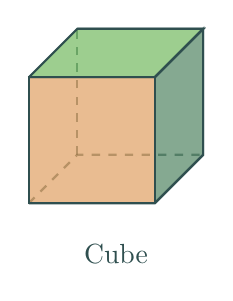
\begin{tikzpicture}[thick,scale=0.8,DarkSlateGray]
    \coordinate (A1) at (-1,-1,-1);
    \coordinate (A2) at (-1,-1,1);
    \coordinate (A3) at (-1,1,-1);
    \coordinate (A4) at (-1,1,1);
    \coordinate (B1) at (1,-1,-1);
    \coordinate (B2) at (1,-1,1);
    \coordinate (B3) at (1,1,-1);
    \coordinate (B4) at (1,1,1);
    % Drawing dashed lines
    \draw[dashed,opacity=0.6] (A2) -- (A1) -- (B1);
    \draw[dashed,opacity=0.6] (A1) -- (A3);
    % Color Faces
    \draw[fill=cof,opacity=0.6]   (A4) -- (B4) -- (B2) -- (A2) ;
    \draw[fill=greet,opacity=0.6]   (B4) -- (B3) -- (B1) -- (B2) ;
    \draw[fill=greeo,opacity=0.6] (A4) -- (B4) -- (B3) -- (A3) ;
    % Drawing Edges
    \draw (A2) -- (B2) -- (B1) ;
    \draw (A2) -- (A4) -- (B4) -- (B2) -- cycle ;
    \draw (A4) -- (A3) -- (B3) -- (B4) ;   
    \draw (B3) -- (B1);
    %
    \node[thick,below=1.5cm] {Cube};
\end{tikzpicture}
% OCTAHEDRON
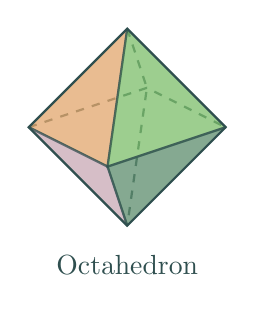
\begin{tikzpicture}[thick,scale=2.5,DarkSlateGray]
    \coordinate (A1) at (0,0);
    \coordinate (A2) at (0.6,0.2);
    \coordinate (A3) at (1,0);
    \coordinate (A4) at (0.4,-0.2);
    \coordinate (B1) at (0.5,0.5);
    \coordinate (B2) at (0.5,-0.5);
    %
    \draw[dashed,opacity=0.6] (A1) -- (A2) -- (A3);        
    \draw[dashed,opacity=0.6] (B1) -- (A2) -- (B2);
    %
    \draw[fill=cof,opacity=0.6] (A1) -- (A4) -- (B1);
    \draw[fill=pur,opacity=0.6] (A1) -- (A4) -- (B2);
    \draw[fill=greeo,opacity=0.6] (A3) -- (A4) -- (B1);
    \draw[fill=greet,opacity=0.6] (A3) -- (A4) -- (B2);
    \draw (B1) -- (A1) -- (B2) -- (A3) --cycle;
    %
    \node[thick,below=1.5cm] at (0.5,0) {Octahedron};
\end{tikzpicture}
% Dodecahedron
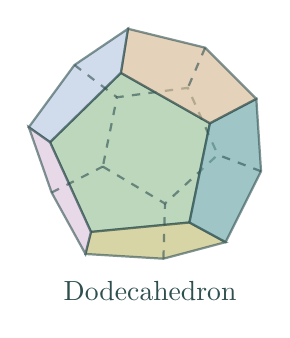
\begin{tikzpicture}[thick,scale=0.5,DarkSlateGray]
    \coordinate (A) at (0,0);
    \coordinate (B) at (2.5,0.24);
    \coordinate (C) at (3.02,2.76);
    \coordinate (D) at (0.76,4.04);
    \coordinate (E) at (-1.04,2.28);
    \coordinate (A1) at (0.3,1.66);
    \coordinate (B1) at (1.88,0.72);
    \coordinate (C1) at (3.22,1.96);
    \coordinate (D1) at (2.46,3.66);
    \coordinate (E1) at (0.66,3.42);
    \coordinate (B2) at (-.14,-.56);
    \coordinate (C2) at (1.84,-.68);
    \coordinate (D2) at (3.42,-.26);
    \coordinate (B3) at (4.32,1.54);
    \coordinate (C3) at (4.2,3.38);
    \coordinate (D3) at (2.9,4.68);
    \coordinate (B4) at (.94,5.16);
    \coordinate (C4) at (-.42,4.24);
    \coordinate (D4) at (-1.58,2.66);
    \coordinate (F) at (-1,1);
    
    \draw[fill=DarkSeaGreen,opacity=0.6] (A)--(B)--(C)--(D)--(E)--cycle;
    \draw[opacity=0.6,dashed] (A1)--(B1)--(C1)--(D1)--(E1)--cycle;
    \draw[fill=DarkKhaki,opacity=0.6] (A)--(B2)--(C2)--(D2)--(B)--cycle;
    \draw[fill=CadetBlue,opacity=0.6] (B)--(D2)--(B3)--(C3)--(C)--cycle;
    \draw[fill=Tan,opacity=0.6] (C)--(C3)--(D3)--(B4)--(D)--cycle;
    \draw[fill=LightSteelBlue,opacity=0.6] (D)--(B4)--(C4)--(D4)--(E)--cycle;
    \draw[fill=Thistle,opacity=0.6] (E)--(D4)--(F)--(B2)--(A)--cycle;
    \path[opacity=0.6] (B2)--(C2)--(B1)--(A1)--(F)--cycle;
    \draw[opacity=0.6,dashed] (C2)--(B1) (F)--(A1);
    \path[opacity=0.6] (C2)--(D2)--(B3)--(C1)--(B1)--cycle;
    \draw[opacity=0.6,dashed] (B3)--(C1);
    \path[opacity=0.6] (B3)--(C3)--(D3)--(D1)--(C1)--cycle;
    \draw[opacity=0.6,dashed] (D3)--(D1);
    \path[opacity=0.6] (D3)--(B4)--(C4)--(E1)--(D1)--cycle;
    \draw[opacity=0.6,dashed] (C4)--(E1);
%titik dengan ball
%http://tex.stackexchange.com/questions/228946/prevent-shifting-of-shading-center-point-when-using-relative-coordinates
    % \shadedraw[ball color=DarkSlateGray!15!white, draw=DarkSlateGray!50] (A) circle (0.08) ;
    % \shadedraw[ball color=DarkSlateGray!15!white, draw=DarkSlateGray!50](B) circle (0.08);
    % \shadedraw[ball color=DarkSlateGray!15!white, draw=DarkSlateGray!50](C) circle (0.08);
    % \shadedraw[ball color=DarkSlateGray!15!white, draw=DarkSlateGray!50](D) circle (0.08);
    % \shadedraw[ball color=DarkSlateGray!15!white, draw=DarkSlateGray!50](E) circle (0.08);
    % \shadedraw[ball color=DarkSlateGray!15!white, draw=DarkSlateGray!50](F) circle (0.08);
    % \shadedraw[ball color=DarkSlateGray!15!white, draw=DarkSlateGray!50] (A1) circle (0.08) ;
    % \shadedraw[ball color=DarkSlateGray!15!white, draw=DarkSlateGray!50](B1) circle (0.08);
    % \shadedraw[ball color=DarkSlateGray!15!white, draw=DarkSlateGray!50](C1) circle (0.08);
    % \shadedraw[ball color=DarkSlateGray!15!white, draw=DarkSlateGray!50](D1) circle (0.08);
    % \shadedraw[ball color=DarkSlateGray!15!white, draw=DarkSlateGray!50](E1) circle (0.08);
    % \shadedraw[ball color=DarkSlateGray!15!white, draw=DarkSlateGray!50](B2) circle (0.08);
    % \shadedraw[ball color=DarkSlateGray!15!white, draw=DarkSlateGray!50](C2) circle (0.08);
    % \shadedraw[ball color=DarkSlateGray!15!white, draw=DarkSlateGray!50](D2) circle (0.08);
    % \shadedraw[ball color=DarkSlateGray!15!white, draw=DarkSlateGray!50](B3) circle (0.08);
    % \shadedraw[ball color=DarkSlateGray!15!white, draw=DarkSlateGray!50](C3) circle (0.08);
    % \shadedraw[ball color=DarkSlateGray!15!white, draw=DarkSlateGray!50](D3) circle (0.08);
    % \shadedraw[ball color=DarkSlateGray!15!white, draw=DarkSlateGray!50](B4) circle (0.081);
    % \shadedraw[ball color=DarkSlateGray!15!white, draw=DarkSlateGray!50](C4) circle (0.08);
    % \shadedraw[ball color=DarkSlateGray!15!white, draw=DarkSlateGray!50](D4) circle (0.08);
   %
    \node[thick,below=0.5cm] at (1.5,0,0) {Dodecahedron};
\end{tikzpicture}
% Icosphedron
    \tdplotsetmaincoords{60}{100}
    \begin{tikzpicture}[tdplot_main_coords,scale=1,line join=round, scale=0.4, DarkSlateGray]
    \pgfmathsetmacro\a{2}
    \pgfmathsetmacro{\phi}{\a*(1+sqrt(5))/2}
    \path 
    coordinate(A) at (0,\phi,\a)
    coordinate(B) at (0,\phi,-\a)
    coordinate(C) at (0,-\phi,\a)
    coordinate(D) at (0,-\phi,-\a)
    coordinate(E) at (\a,0,\phi)
    coordinate(F) at (\a,0,-\phi)
    coordinate(G) at (-\a,0,\phi)
    coordinate(H) at (-\a,0,-\phi)
    coordinate(I) at (\phi,\a,0)
    coordinate(J) at (\phi,-\a,0)
    coordinate(K) at (-\phi,\a,0)
    coordinate(L) at (-\phi,-\a,0); 
    \draw[dashed, thick]    (B) -- (H) -- (F) 
    (D) -- (L) -- (H) --cycle 
    (K) -- (L) -- (H) --cycle
    (K) -- (L) -- (G) --cycle
    (C) -- (L) (B)--(K) (A)--(K)
    ;

        \draw[thick]
        (A) -- (I) -- (B) --cycle 
        (F) -- (I) -- (B) --cycle 
        (F) -- (I) -- (J) --cycle
        (F) -- (D) -- (J) --cycle
        (C) -- (D) -- (J) --cycle
        (C) -- (E) -- (J) --cycle
        (I) -- (E) -- (J) --cycle
        (I) -- (E) -- (A) --cycle
        (G) -- (E) -- (A) --cycle
        (G) -- (E) -- (C) --cycle
        ; 
        \draw[fill=DarkSeaGreen,opacity=0.6] (A) -- (I) -- (B) --cycle ;
        \draw[fill=DarkKhaki,opacity=0.6]  (F) -- (I) -- (B) --cycle ;
        \draw[fill=Tan,opacity=0.6]  (F) -- (I) -- (J) --cycle;
        \draw[fill=CadetBlue,opacity=0.6]  (F) -- (D) -- (J) --cycle;
        \draw[fill=LightYellow,opacity=0.6]    (C) -- (D) -- (J) --cycle;
        \draw[fill=Thistle,opacity=0.6]   (C) -- (E) -- (J) --cycle;
        \draw[fill=DarkGray,opacity=0.6]  (I) -- (E) -- (J) --cycle;
        \draw[fill=LightSteelBlue,opacity=0.6]     (I) -- (E) -- (A) --cycle;
        \draw[fill=DarkSalmon,opacity=0.6]   (G) -- (E) -- (A) --cycle;
        \draw[fill=LightPink,opacity=0.6]    (G) -- (E) -- (C) --cycle;
           %
        \node[thick,below=1.5cm] at (0.7,0,0) {Icosahedron};
\end{tikzpicture}
